\subsection{Calculo de $W_{p}$ correspondiente a cada compuerta NOT}

Se definen tres compuertas NOT en cascada con las características:
\begin{itemize}
    \item $\frac{\beta_{n_1}}{\beta_{p_1}} = 1$
    \item $\frac{\beta_{n_2}}{\beta_{p_2}} = 10$
    \item $\frac{\beta_{n_3}}{\beta_{p_3}} = 0.1$
\end{itemize}

Donde los transistores de la primera compuerta son los mismos que los de la sección \ref{sec:compuerta not}.

Por ende, $W_n = 2 \mu m$ y $W_p = 4.83 \mu m$ para la primera compuerta, considerando la simulación realizada.
Y para las siguientes compuertas, considerando las modificaciones hechas a la primera, serán de $W_{p_2} = 0.483 \mu m$ y $W_{p_3} = 48.3 \mu m$.

\subsection{Simulación de las compuertas NOT}

\begin{figure}[H]
    \centering
    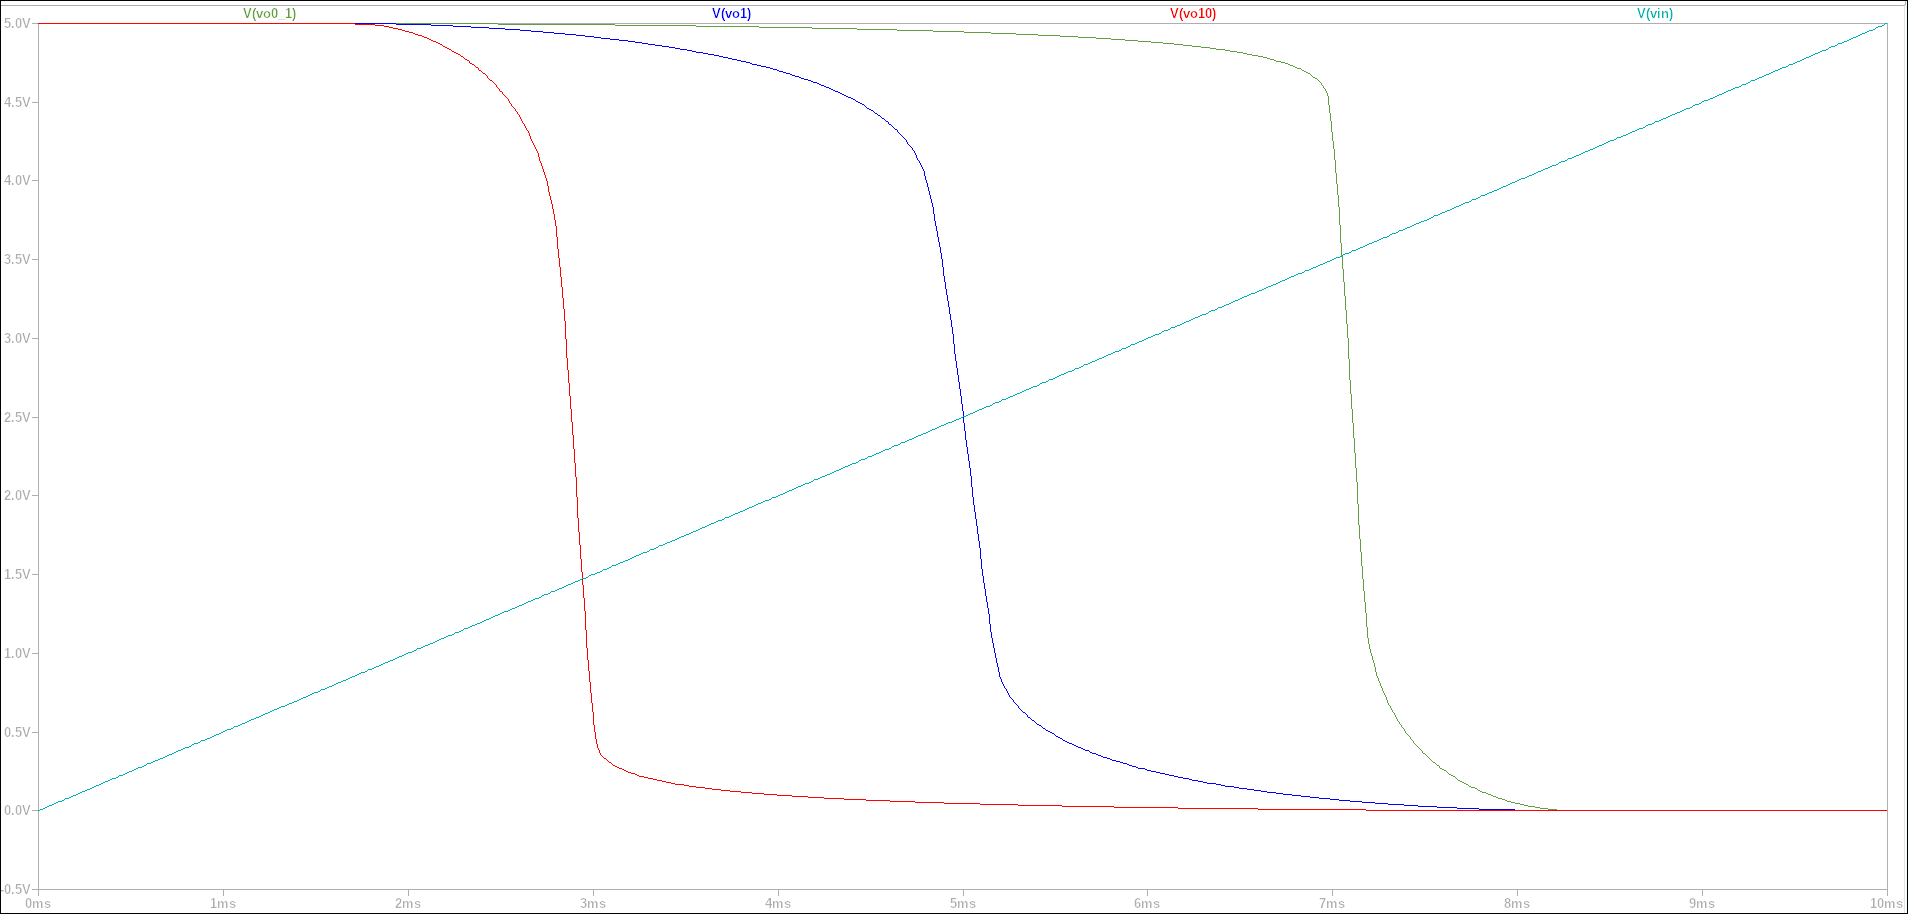
\includegraphics[width=0.8\textwidth]{Imagenes/ej3.png}
    \caption{Simulación de las compuertas NOT con diferentes relaciones $\frac{\beta_n}{\beta_p}$}
    \label{fig:not_simulation}
\end{figure}

\subsection{Márgenes de Ruido}
Los márgenes de ruido se pueden calcular a partir de las curvas de transferencia de las compuertas NOT. Para cada compuerta, se identifican los puntos donde la salida cambia de estado (de alto a bajo o viceversa) y se determinan los niveles de voltaje correspondientes.

\begin{equation}
    NMH = V_{OH} - V_{IH}
\end{equation}
\begin{equation}
    NML = V_{IL} - V_{OL}
\end{equation}

Los puntos de transición se obtienen de encontrar donde la derivada es de módulo unitario.

\begin{table}[H]
    \centering
    \begin{tabular}{l|c|c|c} \hline
    Relación $\frac{\beta_n}{\beta_p}$ & 1 & 10 & 0.1 \\ \hline
    NMH & 1.765 & 3.310 & 3.290 \\ 
    NML & 1.745 & 0.805 & 0.817 \\ \hline
    \end{tabular}
    \caption{Márgenes de ruido para cada compuerta NOT}
    \label{tab:margenes_ruido}
\end{table}

Se puede apreciar de la tabla que el margen de ruido es más simétrico cuánto más cercana a 1 es la relación $\frac{\beta_n}{\beta_p}$. 
Esto se debe a que una relación de 1 implica que los transistores NMOS y PMOS tienen características similares, lo que resulta en una curva de transferencia más equilibrada. 
En cambio, relaciones extremas (10 o 0.1) generan curvas de transferencia más asimétricas, lo que afecta negativamente los márgenes de ruido.
